%**************************************************************
% Lab 12: CPU
%**************************************************************
\chapter{Central Processing Unit}\label{lab12}

\section{Introduction}

\subsection{First Steps}

When building a \ac{CPU}, the first few steps do not involve slinging gates into a circuit. As in most things, planning will save time when executing.

\subsubsection{Purpose}

The first question to answer when building a \ac{CPU} is its purpose. It makes a great deal of difference whether the \ac{CPU} is intended for a single purpose of some sort or a more generalized application. The better the purpose can be defined the simpler (and easier) the designing job becomes. For example, there is no need to design a \ac{CPU} with a lot of ``bells and whistles'' that is intended to be embedded in a microwave oven. A simple 4-bit \ac{CPU} can do that job.

\subsubsection{Instruction Set}

After the \acp{CPU} purpose has been defined, the instruction set must be designed. In general, the fewer instructions that are needed for the \ac{CPU} to do its job, the simpler the design will be. Of course, the designer must include enough instructions to ensure the \ac{CPU} can be effective.\footnote{As an aside, there has been some theoretical work concerning the smallest possible instruction set that can still be used to create a working \ac{CPU}. The current record is one: one instruction is all that is necessary to create a functional \ac{CPU}. While some would argue which instruction is best; in general, computer scientists agree that ``Subtract and Branch if Less Than or Equal to Zero'' is most efficient. To find out more about this type of \ac{CPU}, search for ``SUBLEQ.''}

\subsubsection{States}

The next step is to define the various states the \ac{CPU} can enter and what should happen in each state. While that discussion is beyond the scope of this lesson, in general the \acp{CPU} various functions are mapped out so the designer can create circuits to match each function.

A \acp{CPU} states can be divided into three broad categories: Fetch, Decode, Execute. During the Fetch state, an instruction is fetched from memory and brought into the \ac{CPU}. The instruction is next decoded so the \ac{CPU} knows what type of instruction was fetched. Finally, the microcode steps required by the instruction are executed. The entire cycle repeats until the program is completed. Here is a generic diagram of the instruction cycle:

\bigskip

\smartdiagram[circular diagram:clockwise]{%
	Fetch,Decode,Execute
}

\section{Purpose}

%%%%%%%%%%%%%%%%%%%%%%%%%%%%%%%%%%%%%%%%%%%%%%%%%%%%%%%%%%%%%%
% After I create the CPU I need to start here and update this part of the lab.
%%%%%%%%%%%%%%%%%%%%%%%%%%%%%%%%%%%%%%%%%%%%%%%%%%%%%%%%%%%%%%

A \ac{CPU} contains several components that are tied together with bus lines. Figure \ref{fig:11-01} is a block diagram that shows the main components of the \ac{CPU} being studied in this book: 

\begin{figure}[H]
	\centering
	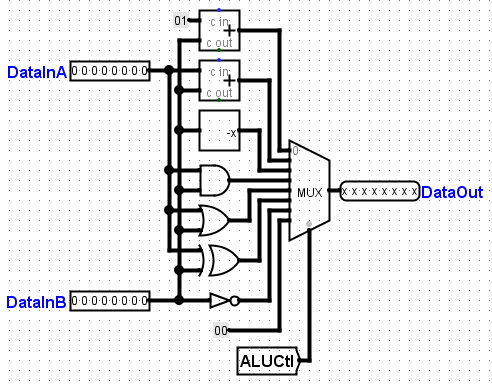
\includegraphics[width=\maxwidth{.95\linewidth}]{gfx/11-01}
	\caption{Simple Processor}
	\label{fig:11-01}
\end{figure}

Here is the purpose for each of these components (from the top of the diagram):

\begin{itemize}
	\item The Ctrl circuit controls all functions within the \ac{CPU}. The output of the Ctrl circuit is placed on the Control Bus where it can then be used to turn on/off various multiplexors and control buffers in order to control the data flow between the components on the data bus. In operation, the \ac{CPU} “fetches” the next program instruction from memory, and then the control circuit interprets that instruction and opens or closes data paths as appropriate.
	\item The Arithmetic Logic Unit (ALU) is responsible for all data manipulation, such as adding two numbers. The ALU sends the results of its work to a register called the Accumulator (which is internal to the ALU on this \ac{CPU}). 
	\item The Gen Regs (General Registers) are a number of registers that are used to temporarily store information while it is being processed. These registers may be considered the “scratch pad” of the \ac{CPU}.
	\item The Pgm Cnter (Program Counter) keeps track of the address of the memory location that contains the next program instruction to be executed. That instruction is then “fetched” and processed by the Ctrl circuit.
	\item The Addr Reg (Address Register) contains a RAM address that is important for the current operation; perhaps, for example, a single byte of an ASCII encoded message that needs to be displayed on the screen. The output of the Address Register is sent directly to RAM through the Address Bus. 
	\item RAM contains the program that is currently being executed. Most of the information traveling on the Data Bus either comes from or is going to RAM.
	\item Peripherals are devices that the \ac{CPU} must control; such as a hard drive or monitor.
\end{itemize}

\footnote{Much of the material in this unit was adapted from a similar lab written by Dr. Lawlor for TKGate, another logic simulator. Here is the URL for that lab: \url{http://www.cs.uaf.edu/2008/fall/cs441/lecture/09_09_\ac{CPU}_construction.html}}

\section{Procedure}










\subsection{Testing the Circuit}

The circuit should be tested by ...

\section{Challenge}

Whatever

\section{Deliverable}

To receive a grade for this lab, build the \ac{CPU} circuit and then complete the Challenge. Be sure the standard identifying information is at the top left of the \ac{CPU} \lstinline{main} circuit, similar to: 

\bigskip
% The minipage environment keeps the three lines together - no page break.
\begin{minipage}{\linewidth}
	\begin{verbatim}
	George Self
	Lab 12: CPU
	April 30, 2018
	\end{verbatim}
\end{minipage}
\bigskip

Save the \ac{CPU} circuit in a file with this name: \textit{Lab12\_CPU}. Complete the code required in the Challenge and store that in a Word or Text file with the name \textit{Lab12\_Code}. Submit both files for grading.

